\section{Analyzer::Base3D Class Reference}
\label{classAnalyzer_1_1Base3D}\index{Analyzer::Base3D@{Analyzer::Base3D}}
{\tt \#include $<$analyzerbase.h$>$}

Inheritance diagram for Analyzer::Base3D:\begin{figure}[H]
\begin{center}
\leavevmode
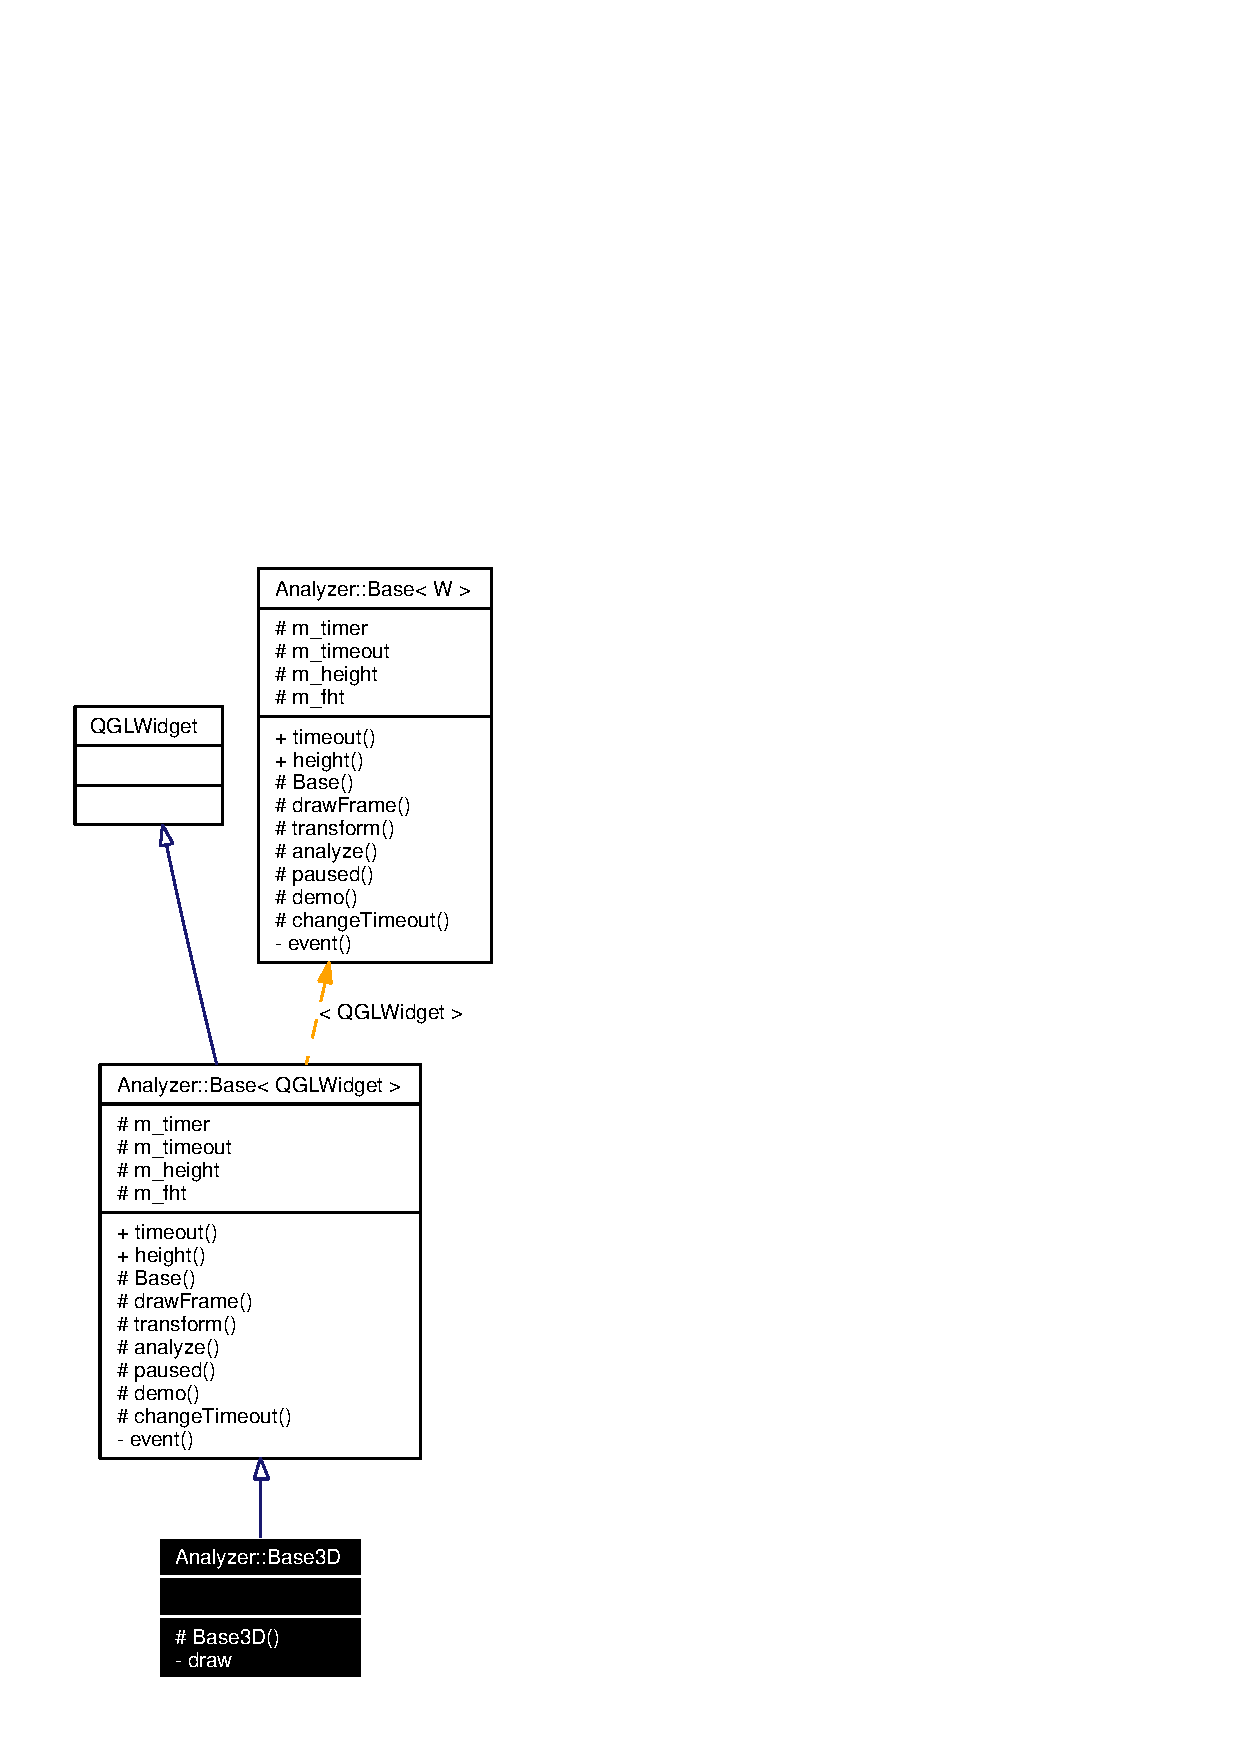
\includegraphics[width=125pt]{classAnalyzer_1_1Base3D__inherit__graph}
\end{center}
\end{figure}
Collaboration diagram for Analyzer::Base3D:\begin{figure}[H]
\begin{center}
\leavevmode
\includegraphics[width=95pt]{classAnalyzer_1_1Base3D__coll__graph}
\end{center}
\end{figure}
\subsection*{Public Member Functions}
\begin{CompactItemize}
\item 
uint {\bf timeout} () const
\item 
uint {\bf height} () const
\end{CompactItemize}
\subsection*{Protected Member Functions}
\begin{CompactItemize}
\item 
{\bf Base3D} ({\bf QWidget} $\ast$w, uint i1, uint i2)
\item 
void {\bf draw\-Frame} ()
\item 
virtual void {\bf transform} ({\bf Scope} \&)
\item 
virtual void {\bf analyze} (const {\bf Scope} \&)=0
\item 
virtual void {\bf paused} ()
\item 
virtual void {\bf demo} ()
\item 
void {\bf change\-Timeout} (uint new\-Timeout)
\end{CompactItemize}
\subsection*{Protected Attributes}
\begin{CompactItemize}
\item 
QTimer {\bf m\_\-timer}
\item 
uint {\bf m\_\-timeout}
\item 
uint {\bf m\_\-height}
\item 
{\bf FHT} {\bf m\_\-fht}
\end{CompactItemize}
\subsection*{Private Slots}
\begin{CompactItemize}
\item 
void {\bf draw} ()
\end{CompactItemize}


\subsection{Constructor \& Destructor Documentation}
\index{Analyzer::Base3D@{Analyzer::Base3D}!Base3D@{Base3D}}
\index{Base3D@{Base3D}!Analyzer::Base3D@{Analyzer::Base3D}}
\subsubsection{\setlength{\rightskip}{0pt plus 5cm}Analyzer::Base3D::Base3D ({\bf QWidget} $\ast$ {\em w}, uint {\em i1}, uint {\em i2})\hspace{0.3cm}{\tt  [inline, protected]}}\label{classAnalyzer_1_1Base3D_Analyzer_1_1Base3Db0}




Definition at line 118 of file analyzerbase.h.



\footnotesize\begin{verbatim}118 : Base<QGLWidget>( w, i1, i2 ) {}
\end{verbatim}\normalsize 


\subsection{Member Function Documentation}
\index{Analyzer::Base3D@{Analyzer::Base3D}!analyze@{analyze}}
\index{analyze@{analyze}!Analyzer::Base3D@{Analyzer::Base3D}}
\subsubsection{\setlength{\rightskip}{0pt plus 5cm}virtual void {\bf Analyzer::Base}$<$ {\bf QGLWidget}  $>$::analyze (const {\bf Scope} \&)\hspace{0.3cm}{\tt  [protected, pure virtual, inherited]}}\label{classAnalyzer_1_1Base_Analyzer_1_1Baseb3}


\index{Analyzer::Base3D@{Analyzer::Base3D}!changeTimeout@{changeTimeout}}
\index{changeTimeout@{changeTimeout}!Analyzer::Base3D@{Analyzer::Base3D}}
\subsubsection{\setlength{\rightskip}{0pt plus 5cm}void {\bf Analyzer::Base}$<$ {\bf QGLWidget}  $>$::change\-Timeout (uint {\em new\-Timeout})\hspace{0.3cm}{\tt  [inline, protected, inherited]}}\label{classAnalyzer_1_1Base_Analyzer_1_1Baseb6}




Definition at line 54 of file analyzerbase.h.



\footnotesize\begin{verbatim}55     {
56         m_timer.changeInterval( newTimeout );
57         m_timeout = newTimeout;
58     }
\end{verbatim}\normalsize 
\index{Analyzer::Base3D@{Analyzer::Base3D}!demo@{demo}}
\index{demo@{demo}!Analyzer::Base3D@{Analyzer::Base3D}}
\subsubsection{\setlength{\rightskip}{0pt plus 5cm}virtual void {\bf Analyzer::Base}$<$ {\bf QGLWidget}  $>$::demo ()\hspace{0.3cm}{\tt  [protected, virtual, inherited]}}\label{classAnalyzer_1_1Base_Analyzer_1_1Baseb5}


\index{Analyzer::Base3D@{Analyzer::Base3D}!draw@{draw}}
\index{draw@{draw}!Analyzer::Base3D@{Analyzer::Base3D}}
\subsubsection{\setlength{\rightskip}{0pt plus 5cm}void Analyzer::Base3D::draw ()\hspace{0.3cm}{\tt  [inline, private, slot]}}\label{classAnalyzer_1_1Base3D_Analyzer_1_1Base3Dk0}




Definition at line 120 of file analyzerbase.h.



\footnotesize\begin{verbatim}120 {}
\end{verbatim}\normalsize 
\index{Analyzer::Base3D@{Analyzer::Base3D}!drawFrame@{drawFrame}}
\index{drawFrame@{drawFrame}!Analyzer::Base3D@{Analyzer::Base3D}}
\subsubsection{\setlength{\rightskip}{0pt plus 5cm}void {\bf Analyzer::Base}$<$ {\bf QGLWidget}  $>$::draw\-Frame ()\hspace{0.3cm}{\tt  [protected, inherited]}}\label{classAnalyzer_1_1Base_Analyzer_1_1Baseb1}


\index{Analyzer::Base3D@{Analyzer::Base3D}!height@{height}}
\index{height@{height}!Analyzer::Base3D@{Analyzer::Base3D}}
\subsubsection{\setlength{\rightskip}{0pt plus 5cm}uint {\bf Analyzer::Base}$<$ {\bf QGLWidget}  $>$::height () const\hspace{0.3cm}{\tt  [inline, inherited]}}\label{classAnalyzer_1_1Base_Analyzer_1_1Basea1}




Definition at line 43 of file analyzerbase.h.



\footnotesize\begin{verbatim}43 { return m_height; }
\end{verbatim}\normalsize 
\index{Analyzer::Base3D@{Analyzer::Base3D}!paused@{paused}}
\index{paused@{paused}!Analyzer::Base3D@{Analyzer::Base3D}}
\subsubsection{\setlength{\rightskip}{0pt plus 5cm}virtual void {\bf Analyzer::Base}$<$ {\bf QGLWidget}  $>$::paused ()\hspace{0.3cm}{\tt  [protected, virtual, inherited]}}\label{classAnalyzer_1_1Base_Analyzer_1_1Baseb4}


\index{Analyzer::Base3D@{Analyzer::Base3D}!timeout@{timeout}}
\index{timeout@{timeout}!Analyzer::Base3D@{Analyzer::Base3D}}
\subsubsection{\setlength{\rightskip}{0pt plus 5cm}uint {\bf Analyzer::Base}$<$ {\bf QGLWidget}  $>$::timeout () const\hspace{0.3cm}{\tt  [inline, inherited]}}\label{classAnalyzer_1_1Base_Analyzer_1_1Basea0}




Definition at line 42 of file analyzerbase.h.



\footnotesize\begin{verbatim}42 { return m_timeout; }
\end{verbatim}\normalsize 
\index{Analyzer::Base3D@{Analyzer::Base3D}!transform@{transform}}
\index{transform@{transform}!Analyzer::Base3D@{Analyzer::Base3D}}
\subsubsection{\setlength{\rightskip}{0pt plus 5cm}virtual void {\bf Analyzer::Base}$<$ {\bf QGLWidget}  $>$::transform ({\bf Scope} \&)\hspace{0.3cm}{\tt  [protected, virtual, inherited]}}\label{classAnalyzer_1_1Base_Analyzer_1_1Baseb2}




\subsection{Member Data Documentation}
\index{Analyzer::Base3D@{Analyzer::Base3D}!m_fht@{m\_\-fht}}
\index{m_fht@{m\_\-fht}!Analyzer::Base3D@{Analyzer::Base3D}}
\subsubsection{\setlength{\rightskip}{0pt plus 5cm}{\bf FHT} {\bf Analyzer::Base}$<$ {\bf QGLWidget}  $>$::{\bf m\_\-fht}\hspace{0.3cm}{\tt  [protected, inherited]}}\label{classAnalyzer_1_1Base_Analyzer_1_1Basep3}




Definition at line 67 of file analyzerbase.h.\index{Analyzer::Base3D@{Analyzer::Base3D}!m_height@{m\_\-height}}
\index{m_height@{m\_\-height}!Analyzer::Base3D@{Analyzer::Base3D}}
\subsubsection{\setlength{\rightskip}{0pt plus 5cm}uint {\bf Analyzer::Base}$<$ {\bf QGLWidget}  $>$::{\bf m\_\-height}\hspace{0.3cm}{\tt  [protected, inherited]}}\label{classAnalyzer_1_1Base_Analyzer_1_1Basep2}




Definition at line 66 of file analyzerbase.h.\index{Analyzer::Base3D@{Analyzer::Base3D}!m_timeout@{m\_\-timeout}}
\index{m_timeout@{m\_\-timeout}!Analyzer::Base3D@{Analyzer::Base3D}}
\subsubsection{\setlength{\rightskip}{0pt plus 5cm}uint {\bf Analyzer::Base}$<$ {\bf QGLWidget}  $>$::{\bf m\_\-timeout}\hspace{0.3cm}{\tt  [protected, inherited]}}\label{classAnalyzer_1_1Base_Analyzer_1_1Basep1}




Definition at line 65 of file analyzerbase.h.\index{Analyzer::Base3D@{Analyzer::Base3D}!m_timer@{m\_\-timer}}
\index{m_timer@{m\_\-timer}!Analyzer::Base3D@{Analyzer::Base3D}}
\subsubsection{\setlength{\rightskip}{0pt plus 5cm}QTimer {\bf Analyzer::Base}$<$ {\bf QGLWidget}  $>$::{\bf m\_\-timer}\hspace{0.3cm}{\tt  [protected, inherited]}}\label{classAnalyzer_1_1Base_Analyzer_1_1Basep0}




Definition at line 64 of file analyzerbase.h.

The documentation for this class was generated from the following file:\begin{CompactItemize}
\item 
{\bf analyzerbase.h}\end{CompactItemize}
